\section{Performance Evaluation}\label{sec:performance evaluation}

This section evaluates FDWZ and MRCZ in terms of rate--distortion performance, end-to-end data-movement time, parallel throughput, and spatial reconstruction error. We compare them with five representative error-bounded lossy compressors across eight high-order element datasets produced by NekRS, MFEM, and Nektar++.

\subsection{Experimental Setup}\label{sec:performance evaluation:setup}

\subsubsection{Evaluation Platform}\mbox{}

The experiments were conducted on Purdue Anvil. Each compute node contains two 64-core AMD EPYC 7763 processors, for a total of 128 physical CPU cores, and approximately 256~GB of main memory. Datasets~1--3 and~6--8 use one CPU core and one partition, Dataset~4 uses 64 CPU cores and 64 partitions, and Dataset~5 uses 128 CPU cores and 128 partitions. All implementations other than SPERR were compiled with GCC 11.2.0 using \verb|-Ofast -march=native|. SPERR was built separately using its default configuration. For parallel runs, OpenMP threads were bound to physical cores using \verb|OMP_PLACES=cores| and \verb|OMP_PROC_BIND=spread|.

\subsubsection{High-Order Element Datasets}\mbox{}

\begin{table*}[htb]
    \centering
    \caption{High-order element datasets used for evaluating FDWZ, MRCZ, and the baseline compressors.}
    \label{tab:datasets}
    \begin{tabular}{c|ccclc}\toprule
         \textbf{Index} & \textbf{Framework} & \textbf{Element Shape} & \textbf{Number of Elements} & \textbf{Non-constant Fields} & \textbf{Data Type} \\
         \midrule
         1              & NekRS              & $8\times8\times1$      & 1600                        & UX, UY, P, T, S00, S01       & Float \\
         2              & NekRS              & $6\times6\times6$      & 512                         & UZ, T, S00, S01              & Float \\
         3              & NekRS              & $8\times8\times8$      & 512                         & UX, UY, UZ                   & Double \\
         4              & NekRS              & $8\times8\times8$      & 1947154                     & UX, UY, UZ, P, T             & Float \\
         5              & NekRS              & $10\times10\times10$   & 3240264                     & UX, UY, UZ, P, S00           & Float \\
         6              & MFEM               & $21\times21\times1$    & 80                          & One field                    & Double \\
         7              & MFEM               & $5\times5\times1$      & 20480                       & One field                    & Double\\
         8              & Nektar++           & $8\times8\times1$      & 782                         & U, V, P                      & Double\\\bottomrule
    \end{tabular}
\end{table*}

Datasets~1--5 were provided by domain scientists and generated with NekRS~\cite{fischer2022nekrs}; Datasets~6--8 were generated from MFEM~\cite{kolev2010modular} and Nektar++~\cite{moxey2020nektar++} examples. For brevity, a field is denoted by its dataset index followed by its name; for example, 4T denotes the $T$ field of Dataset~4.

\subsubsection{Baseline Compressors}\mbox{}

We evaluate the official APIs of SZ3~\cite{liang2022sz3,zhao2021optimizing}, SZ2~\cite{tao2017significantly}, QoZ~\cite{liu2024high}, ZFP~\cite{lindstrom2014fixed}, and SPERR~\cite{li2023lossy}. Together, they represent interpolation-based, regression-based, block-transform, and wavelet-based compression. Because these APIs operate on regular arrays, their performance on high-order element data depends on how the element tensors are presented to them.

Following the logical representation in Section~\ref{sec:problem formulation:data characteristics}, a partition containing $E_p$ elements is a slice of $X$ with shape $[E_p,n_x,n_y,n_z]$. Let $n=n_xn_yn_z$ denote the number of values per element. Table~\ref{tab:baseline-layouts} defines the five candidate layouts. The 1D, 2D, fused 3D, and 4D layouts each invoke the compressor once per partition. The per-element 3D layout instead invokes it once per element and concatenates the resulting bitstreams.

\begin{table}[htb]
    \centering
    \caption{Candidate layouts for the baseline compressors.}
    \label{tab:baseline-layouts}
    \footnotesize
    \setlength{\tabcolsep}{4pt}
    \begin{tabular*}{\columnwidth}{@{\extracolsep{\fill}}ll@{}}
        \toprule
        Layout & Arrays passed to the compressor \\
        \midrule
        1D & One $[E_pn]$ array \\
        2D & One $[E_p,n]$ array \\
        Fused 3D & One $[E_pn_x,n_y,n_z]$ array \\
        Per-element 3D & $E_p$ arrays of shape $[n_x,n_y,n_z]$ \\
        4D & One $[E_p,n_x,n_y,n_z]$ array \\
        \bottomrule
    \end{tabular*}
\end{table}

SZ3, SZ2, QoZ, and ZFP support all five layouts. SPERR has no 1D or 4D API and is therefore evaluated with only the 2D and two 3D layouts.

\subsection{Storage Reduction Evaluation}

We evaluate every supported layout on Datasets~1--3 and~6--8, compare BR over the common PSNR range of the resulting rate--distortion curves, and select one layout for each compressor. Per-element 3D is generally less effective because it creates many independent bitstreams, repeats metadata, and cannot exploit redundancy across elements. The selected baselines are SZ3-4D, SZ2-3D-fused, QoZ-4D, ZFP-3D-fused, and SPERR-2D. We fix these choices before running Datasets~4 and~5.

\begin{figure*}[htb]
    \centering
    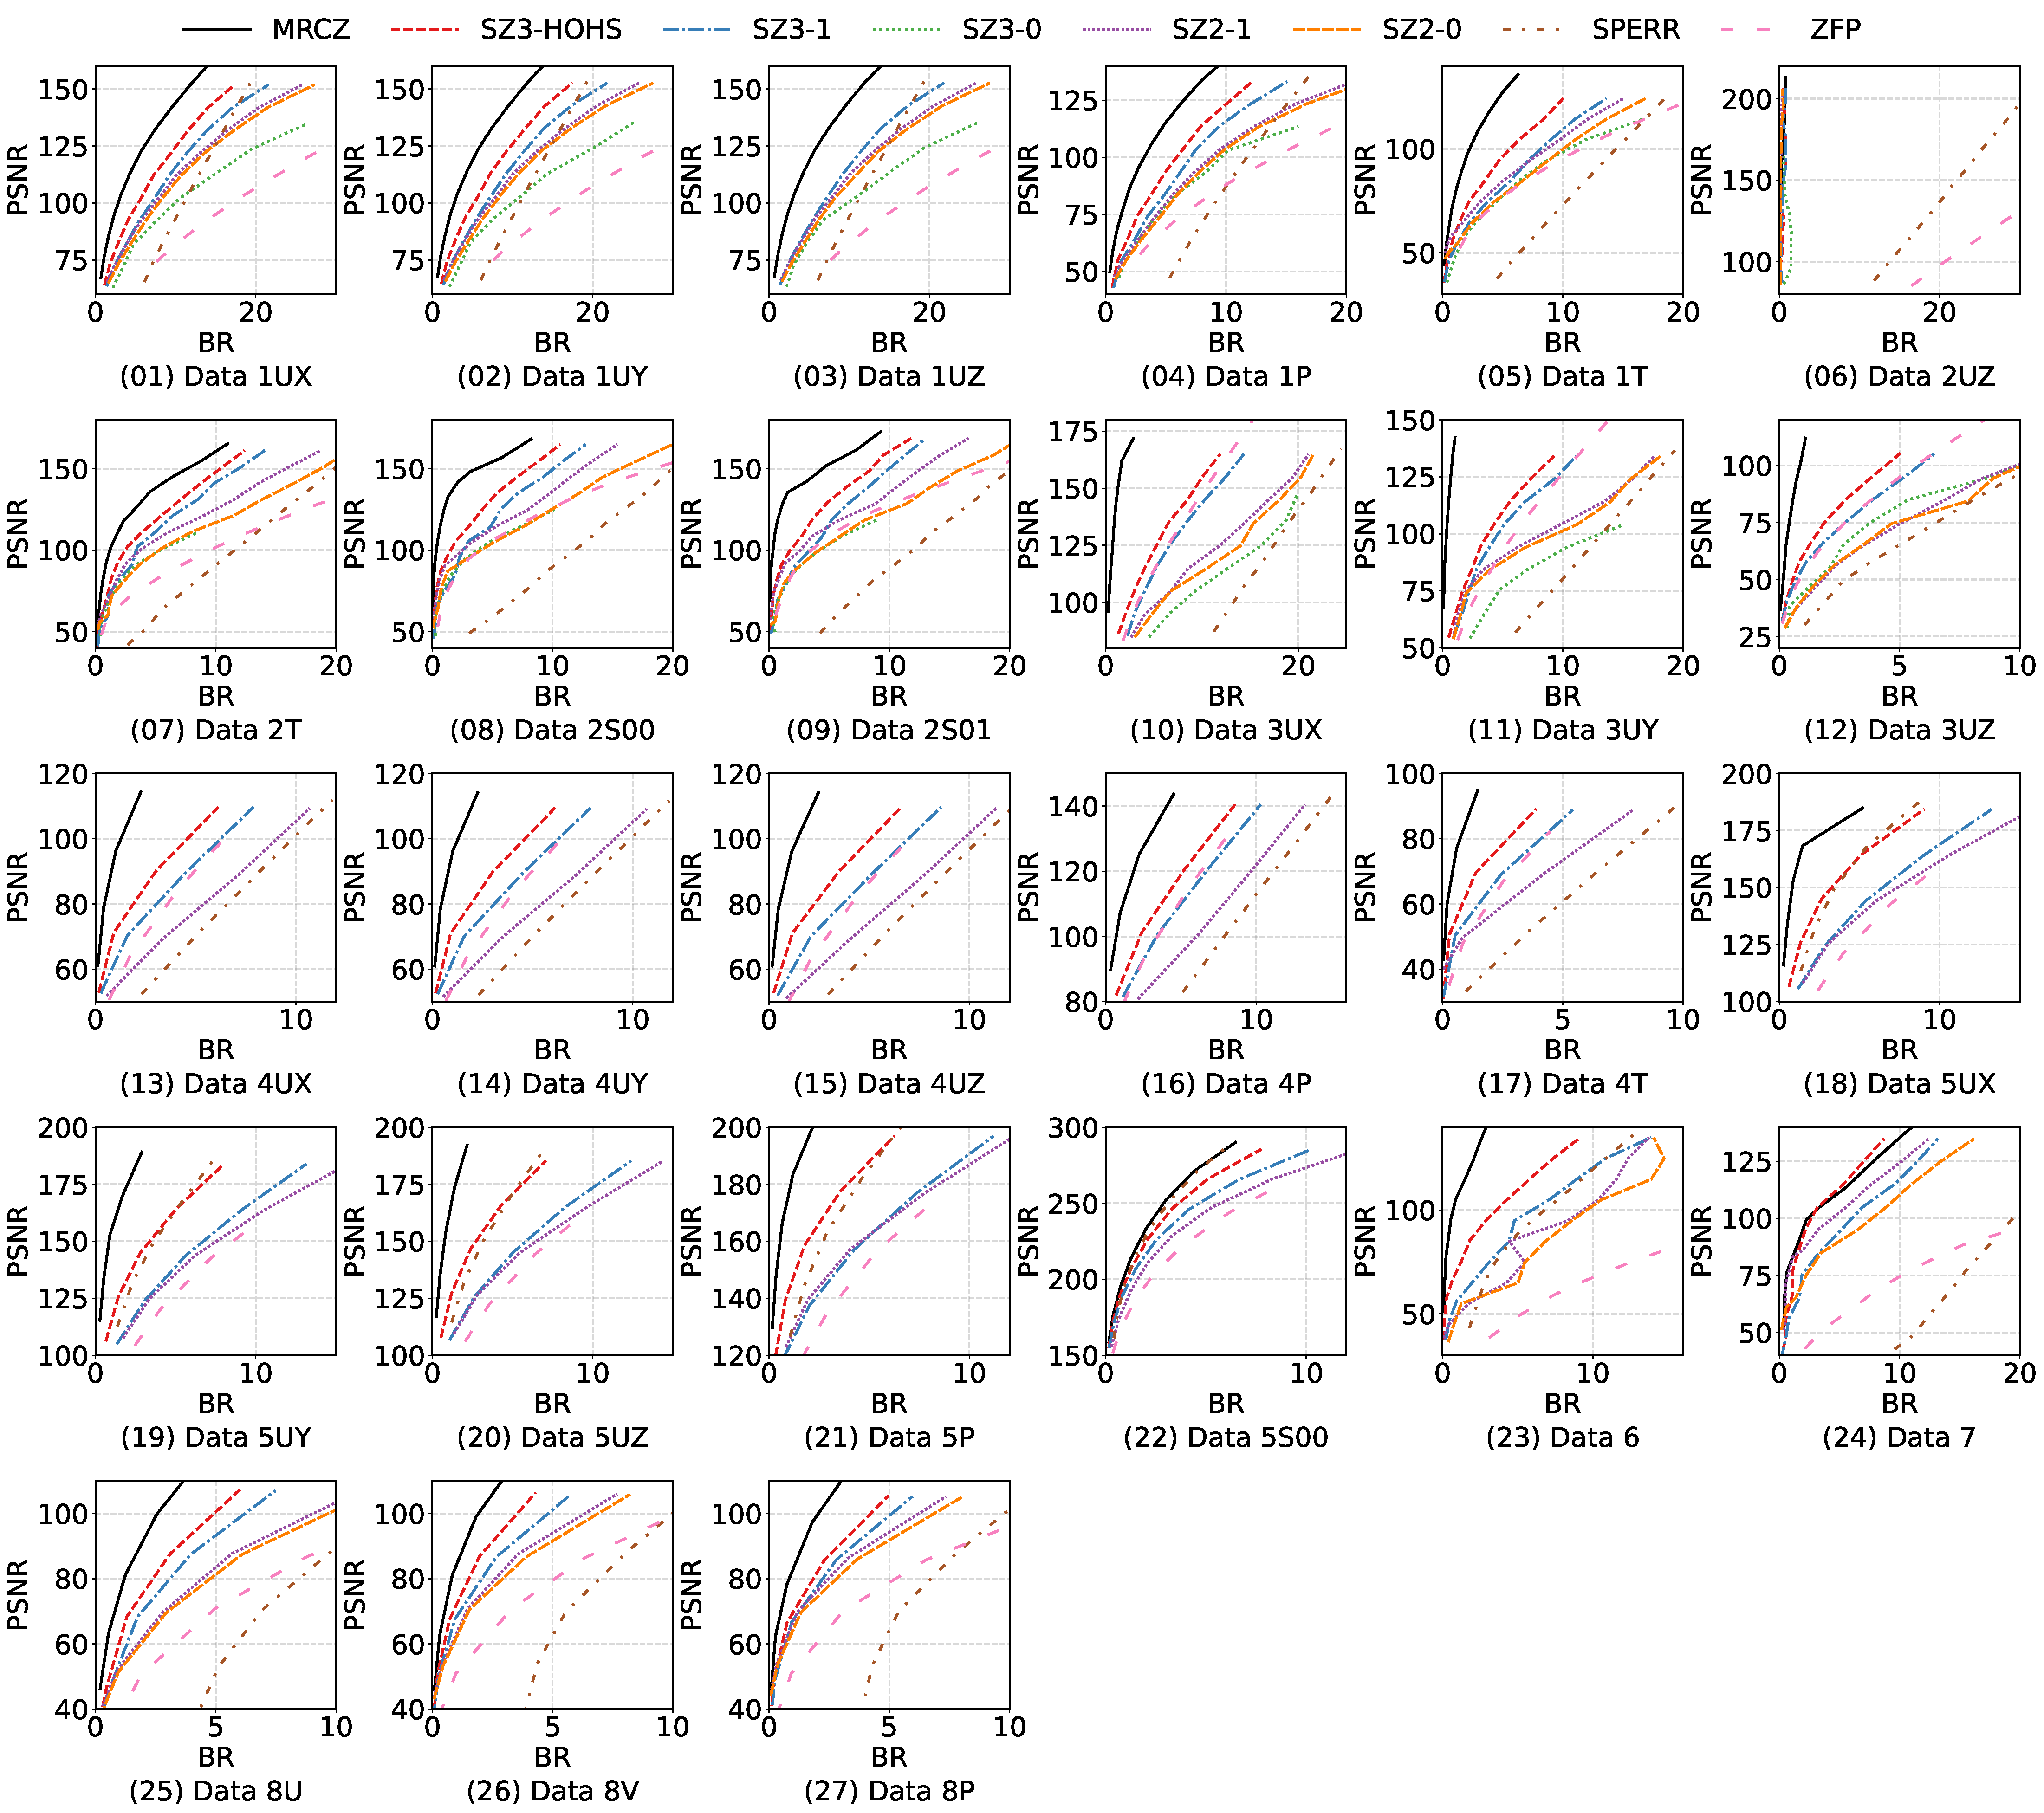
\includegraphics[width=1\textwidth]{figs/7/rd.pdf}
    \caption{Rate--distortion comparison of FDWZ, MRCZ, and the baseline compressors.}
    \label{fig:rate-distortion}
\end{figure*}

Figure~\ref{fig:rate-distortion} presents the rate-distortion curves for all fields in Table~\ref{tab:datasets} across all evaluated compressors. These curves are used to evaluate storage reduction under comparable data quality. The X-axis shows the bit rate, measured in bits per data point. A lower bit rate indicates a smaller compressed representation. The Y-axis shows PSNR, where a higher value indicates lower overall distortion. Therefore, for a fixed PSNR, a curve farther to the left indicates better storage reduction. Equivalently, for a fixed bit rate, a curve higher on the plot indicates better reconstruction quality. Overall, better performance is indicated by curves closer to the upper-left.

Overall, \textbf{\textit{FDWZ and MRCZ consistently outperform all baseline lossy compressors}}. MRCZ achieves the best rate-distortion performance for 26 out of 27 high-order element fields, while FDWZ achieves the second-best curve for 23 out of 27 fields. These results demonstrate that, compared with the baseline compressors, the proposed methods consistently provide greater storage reduction while maintaining comparable reconstruction quality across diverse high-order element datasets.

The performance improvements originate from different design mechanisms in the two proposed methods.
FDWZ achieves better performance by employing distance-weighted interpolation based on the GLL point distribution in the reference element, leading to more accurate predictions.
MRCZ improves compressibility by using a more effective transform that produces more concentrated coefficients. This allows MRCZ to use a smaller coefficient error bound without introducing excessive coefficient-storage overhead. Meanwhile, a smaller coefficient error bound improves the inverse-transform reconstruction accuracy, producing smaller and more concentrated residuals that are easier to compress. Finally, MRCZ reorganizes the quantized coefficients across elements to improve their continuity before lossless encoding, further reducing the final bit rate.

% Some baseline compressors also produce less stable rate-distortion curves. For example, on dataset 6, SZ2-0 and SZ2-1 occasionally increase bit rate while reducing PSNR. In contrast, FDWZ and MRCZ produce smoother and more predictable rate-distortion curves across diverse high-order element fields.

To further quantify storage reduction under practical error-bound settings, we report compression ratios for two representative fields, 4UX (3.71 GB) and 5P (12.07 GB), in Table~\ref{tab:compression-ratios}. Unlike the rate-distortion curves in Figure~\ref{fig:rate-distortion}, which compare methods under PSNR-based reconstruction quality, this table evaluates compression ratios under fixed pointwise error bounds. Due to the different value ranges of the two fields, they are evaluated under different absolute error bounds. We report SZ3-1 and SZ2-1 as the adapted SZ baselines, while omitting SZ3-0 and SZ2-0 due to their poor rate-distortion performance.

\begin{table*}[h]
    \centering
    \caption{Compression ratios of two leading fields 4UX and 5P across all evaluated lossy compressors. The SZ3-0 and SZ2-0 are excluded due to sacrificed performance. The \textbf{highest} and \underline{second-highest} compression ratios are highlighted.}
    \label{tab:compression-ratios}
    \begin{tabular}{c|c|cccccccc}\toprule
        \textbf{Field} & \textbf{Error Bound} & \textbf{MRCZ}    & \textbf{FDWZ} & \textbf{SZ3-1}   & \textbf{SZ2-1}  & \textbf{SPERR}  & \textbf{ZFP} \\
        \midrule
        4UX                     & ABS 1E-1   & \textbf{255.387} & \underline{191.789}  & 118.431 & 57.841 & 13.891 & 7.697\\
        4UX                     & ABS 1E-2   & \textbf{79.910}  & \underline{34.870}   & 20.134  & 9.435  & 6.098  & 4.855\\
        4UX                     & ABS 1E-3   & \textbf{31.391}  & \underline{10.625}   & 7.092   & 4.440  & 3.770  & 3.414\\
        \midrule
        5P                      & ABS 1E-4   & \textbf{196.138} & \underline{97.935}   & 44.649  & 37.830 & 30.479 & 5.932\\
        5P                      & ABS 1E-5   & \textbf{92.083}  & \underline{39.329}   & 15.864  & 16.587 & 17.871 & 3.952\\
        5P                      & ABS 1E-6   & \textbf{48.883}  & \underline{18.094}   & 7.557   & 7.871  & 10.999 & 2.788\\\bottomrule
    \end{tabular}
\end{table*}

Table~\ref{tab:compression-ratios} shows the storage-reduction performance under fixed error-bound constraints. We can find that \textbf{\textit{MRCZ and FDWZ consistently achieve the highest compression ratios across all reported cases.}} MRCZ achieves up to 5.47$\times$ higher compression ratio than SZ3-1, the strongest baseline in this comparison, while FDWZ consistently delivers the second-best compression ratios. These results show that the proposed methods are effective not only under PSNR-based rate-distortion evaluation, but also under the pointwise error-bound settings.

\subsection{End-to-End Workflow Evaluation}

In this subsection, we assess the practical impact of compression on end-to-end data movement between Purdue Anvil and Argonne Bebop using Globus~\cite{chard2017globus}, a widely used service for high-performance data transfer. For each evaluation, we compress all non-constant fields from Datasets~4 and~5 (Table~\ref{tab:datasets}) under an absolute error bound of $10^{-6}$, transfer the compressed data, and decompress it at the destination. The measured end-to-end time captures the trade-off between reduced transfer volume and compression/decompression overhead. Each dataset is evaluated three times, and the average results are reported.


\begin{figure}[htb]
    \centering
    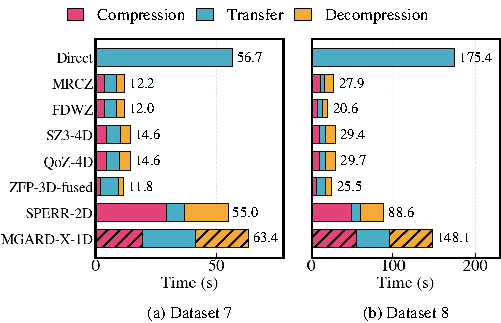
\includegraphics[width=1\linewidth]{figs/7/e2e_time.pdf}
    \caption{End-to-end Workflow Execution Time via Globus}
    \label{fig:transfer}
\end{figure}

As shown in Figure~\ref{fig:transfer}, MRCZ and FDWZ achieve the best end-to-end performance for Data 4 and Data 5, respectively, due to their high compression ratios and efficient implementations. For Data 4, MRCZ and FDWZ achieve end-to-end transfer times of 11.91 and 12.04 seconds, respectively. For Data 5, FDWZ is significantly faster than the other evaluated methods, requiring only 38.32 seconds, because it combines a high compression ratio with low computational overhead. \textit{\textbf{Overall, these results demonstrate the strong capability of FDWZ and MRCZ to reduce data-movement overhead for cross-facility scientific workloads.}}

\subsection{Parallel Throughput}\label{sec:parallel-throughput}

Following the end-to-end workflow evaluation, we further isolate the compression and decompression stages to examine their parallel scalability. Specifically, we conduct a strong-scaling evaluation of OpenMP compression and decompression throughput across all non-constant fields of Datasets 4 and 5 under an absolute error bound of $10^{-6}$. The number of threads is increased up to 128 while the input data size remains fixed. Each field is evaluated three times at each thread count, and we report the harmonic mean of all measured throughput values. Because all fields within each dataset have the same size, this is equivalent to dividing the aggregate processed data size by the aggregate execution time.

\begin{figure}[htb]
    \centering
    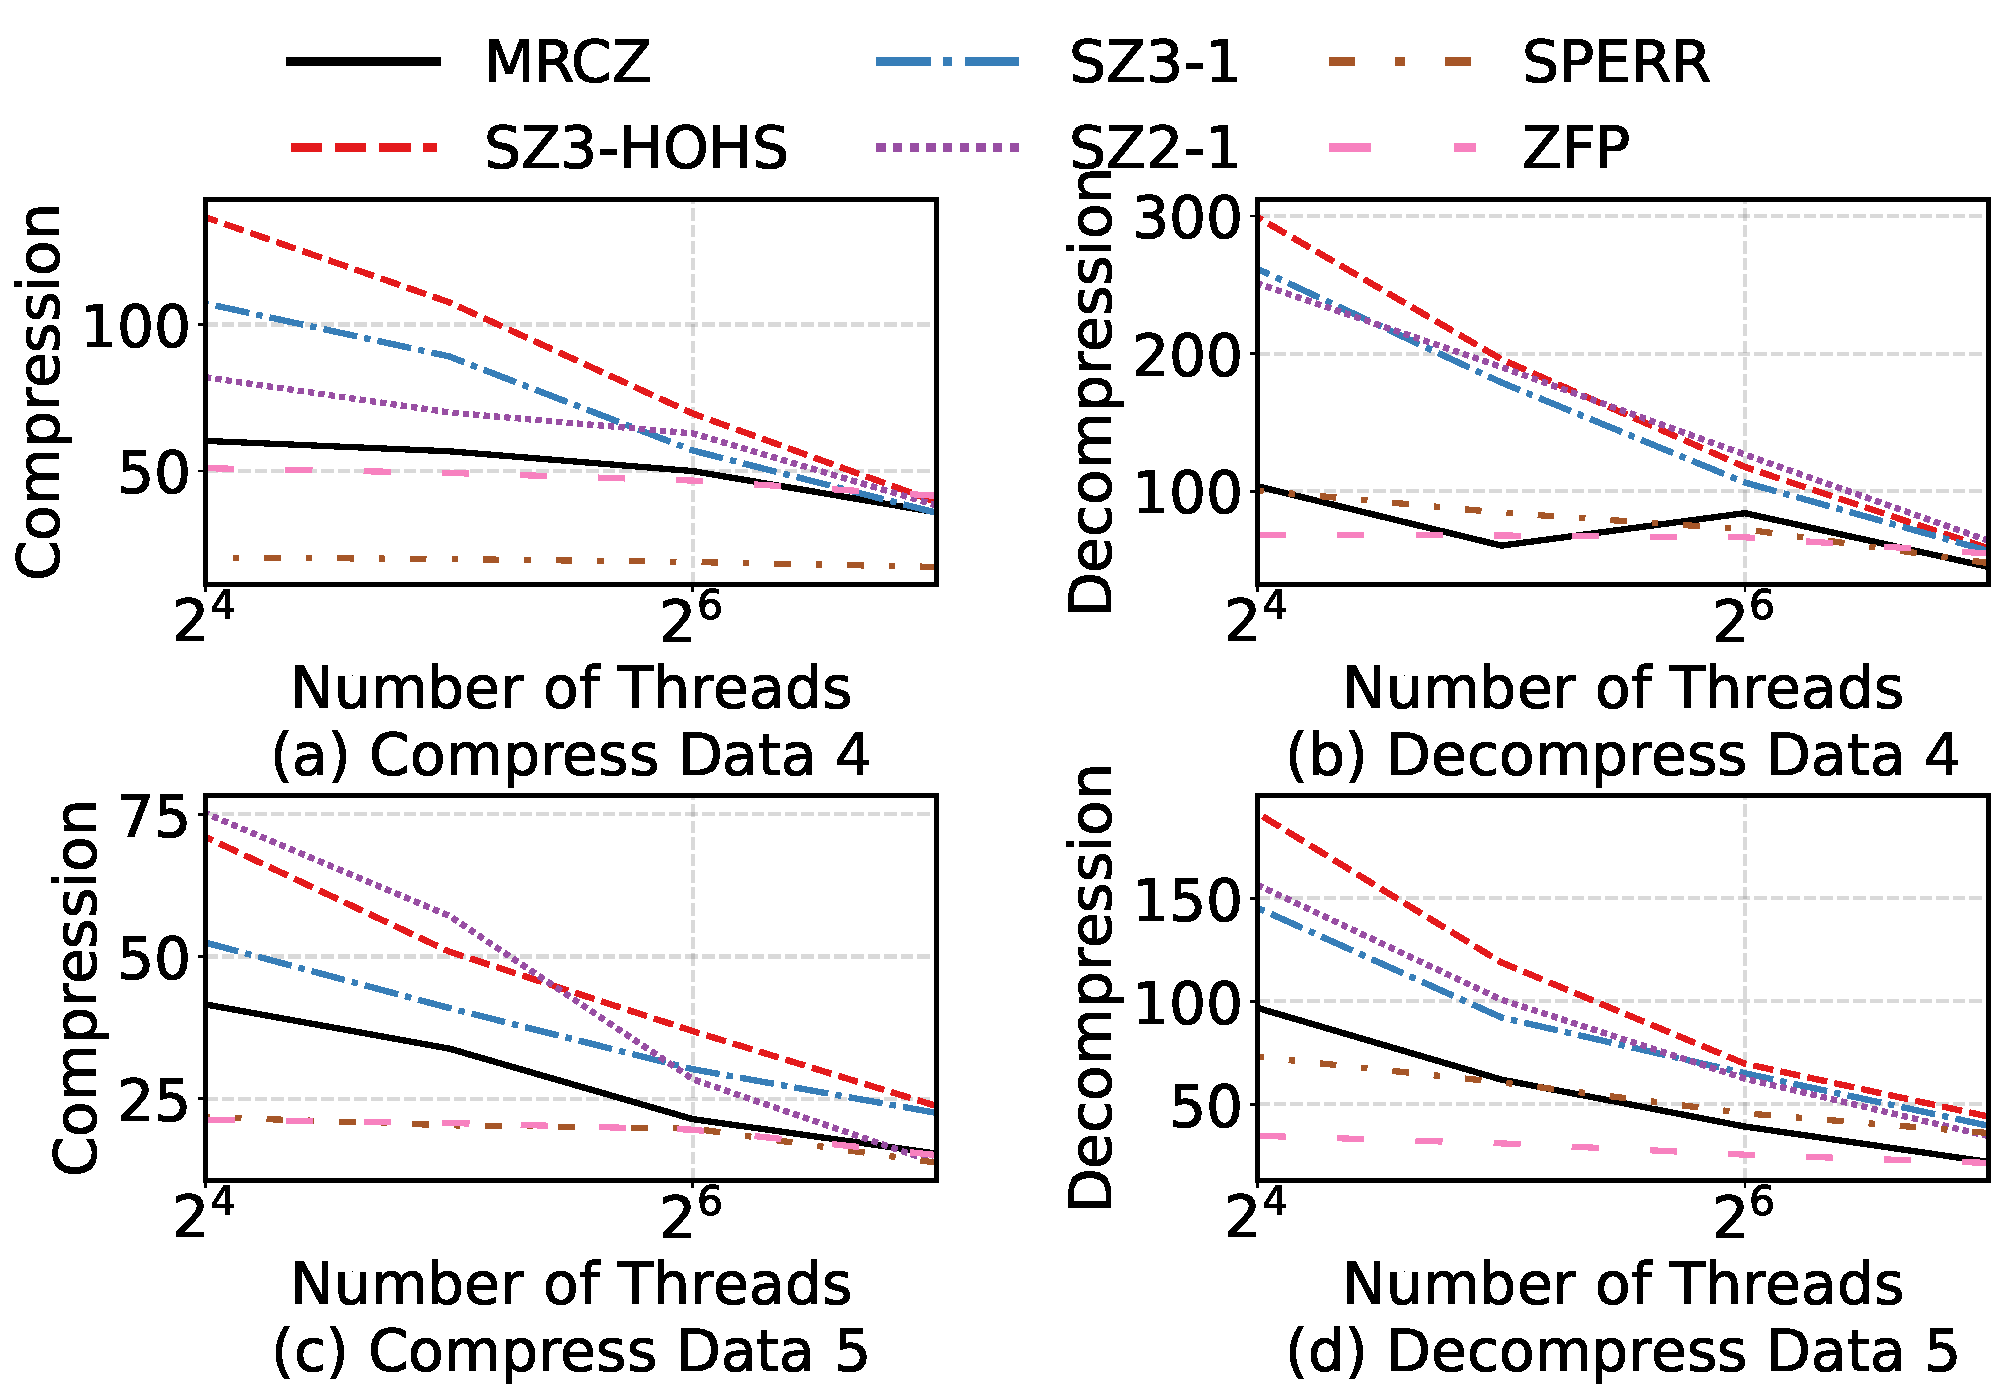
\includegraphics[width=0.9\linewidth]{figs/8-fig9.pdf}
    \caption{Parallel Execution Throughput (MB/s)}
    \label{fig:throughput}
\end{figure}

The results are shown in Figure~\ref{fig:throughput}. \textit{\textbf{FDWZ achieves the highest overall throughput, particularly during decompression, while MRCZ remains competitive despite its more computationally intensive transform-based prediction.}} For example, with 16 threads on Dataset~4, FDWZ and MRCZ achieve per-thread compression throughputs of 136.55 and 60.33 MB/s, respectively. By comparison, SZ3-1, SZ2-1, SPERR, and ZFP achieve 107.18, 82.01, 20.57, and 51.01 MB/s, respectively. MRCZ therefore provides substantially higher throughput than SPERR and moderately higher throughput than ZFP, while also delivering a higher compression ratio. One contributing factor is its accurate prediction, which produces more concentrated quantization symbols and reduces the cost of the subsequent lossless encoding stage.

These results reveal a practical trade-off between compression effectiveness and computational performance. MRCZ is preferable when maximizing compression ratio is the primary objective, whereas FDWZ offers a stronger balance between compression ratio and throughput when execution time is more important.

As the thread count increases, the per-thread throughput of MRCZ, SPERR, and ZFP remains relatively stable because their higher arithmetic intensity makes them less sensitive to shared memory bandwidth. In contrast, the lightweight prediction in FDWZ becomes memory-bandwidth-bound at relatively small thread counts, causing its per-thread throughput to decrease even as aggregate throughput continues to improve.

\subsection{Visualization}\label{sec:performance evaluation:visualization}

In this part, we examine a slice of the temperature field from Dataset~4 (4T in Table~\ref{tab:datasets}). To assess reconstruction quality across different error-bounded lossy compressors, we plot the pointwise absolute reconstruction errors produced by each method. Lighter colors indicate smaller errors and therefore higher reconstruction fidelity. For a fair comparison, all compressors are evaluated at comparable compression ratios close to 26.07. Only a small spatial region is shown for clarity.

\begin{table}[htb]
    \centering
    \caption{Error bounds at a compression ratio of $\sim$26.07.}
    \label{tab:error-bound-visualization}
    \begin{tabular}{c|ccc}
        \toprule
        \textbf{Compressor} & \textbf{MRCZ} & \textbf{FDWZ} & \textbf{SZ3-1} \\
        \textbf{Relative Error Bound} & $1.04\times10^{-4}$ & $7.9\times10^{-4}$ & $2\times10^{-3}$ \\
        \midrule
        \textbf{Compressor} & \textbf{SZ2-1} & \textbf{ZFP} & \textbf{SPERR} \\
        \textbf{Relative Error Bound} & $4.2\times10^{-3}$ & $3.16\times10^{-1}$ & $4.52\times10^{-2}$ \\\bottomrule
    \end{tabular}
\end{table}

\begin{figure}[htb]
  \centering
  \begin{subfigure}[t]{0.45\linewidth}
    \centering
    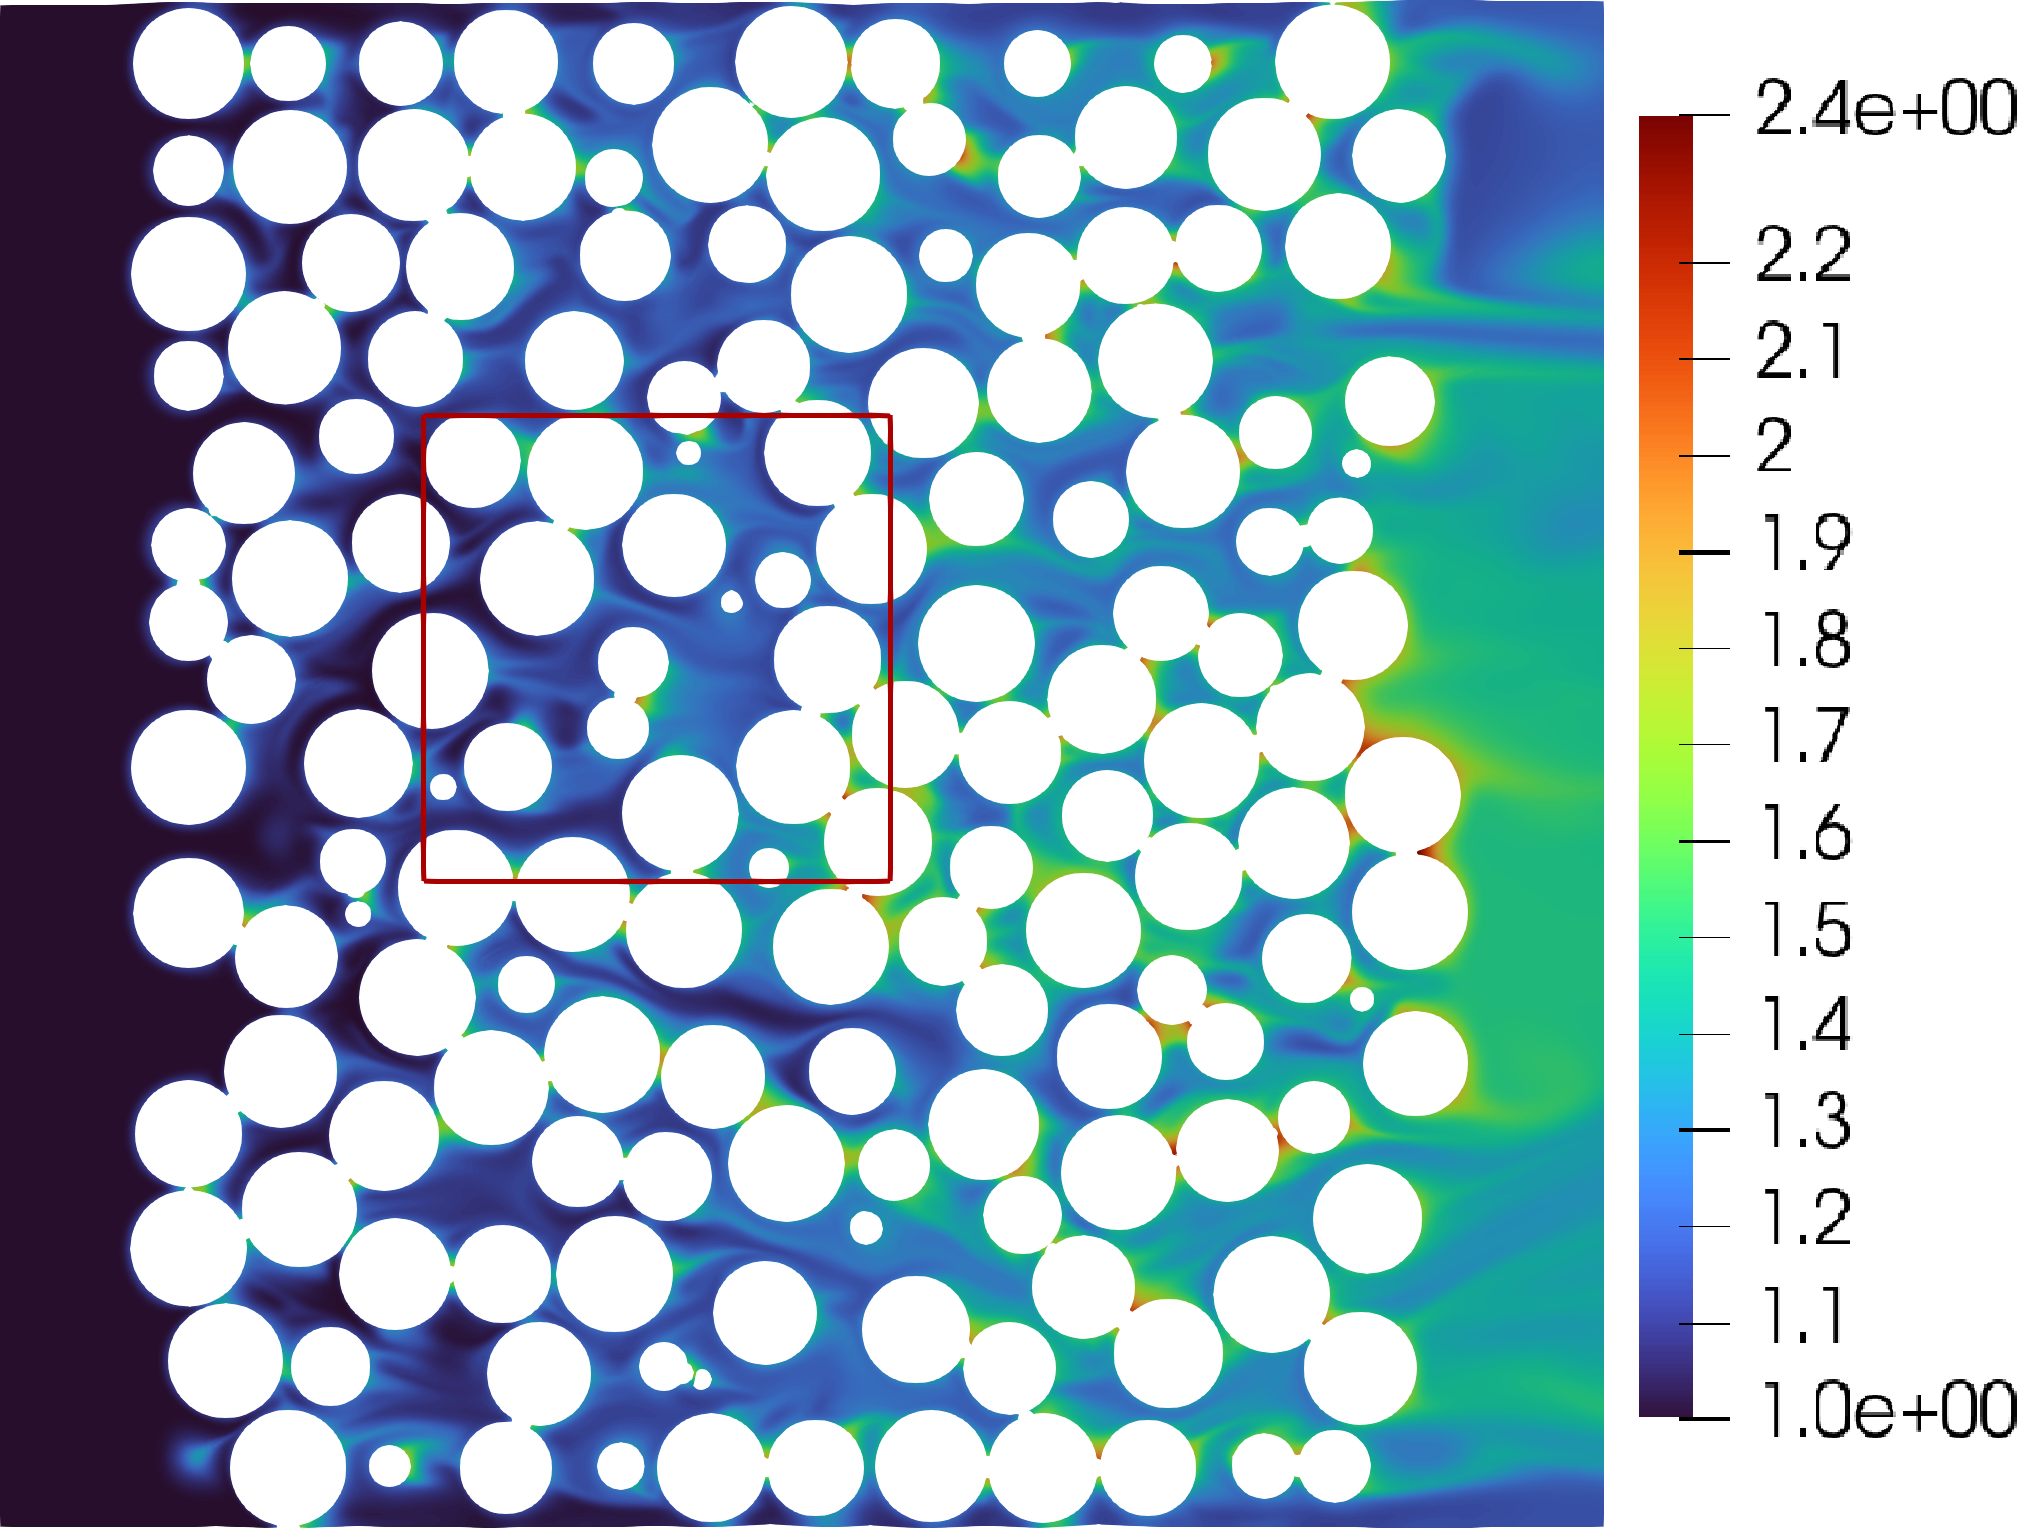
\includegraphics[width=\linewidth]{figs/7/pb0.png}
    \caption{Slice Visualization from 4T}
  \end{subfigure}
  \\
  \begin{subfigure}[t]{0.30\linewidth}
    \centering
    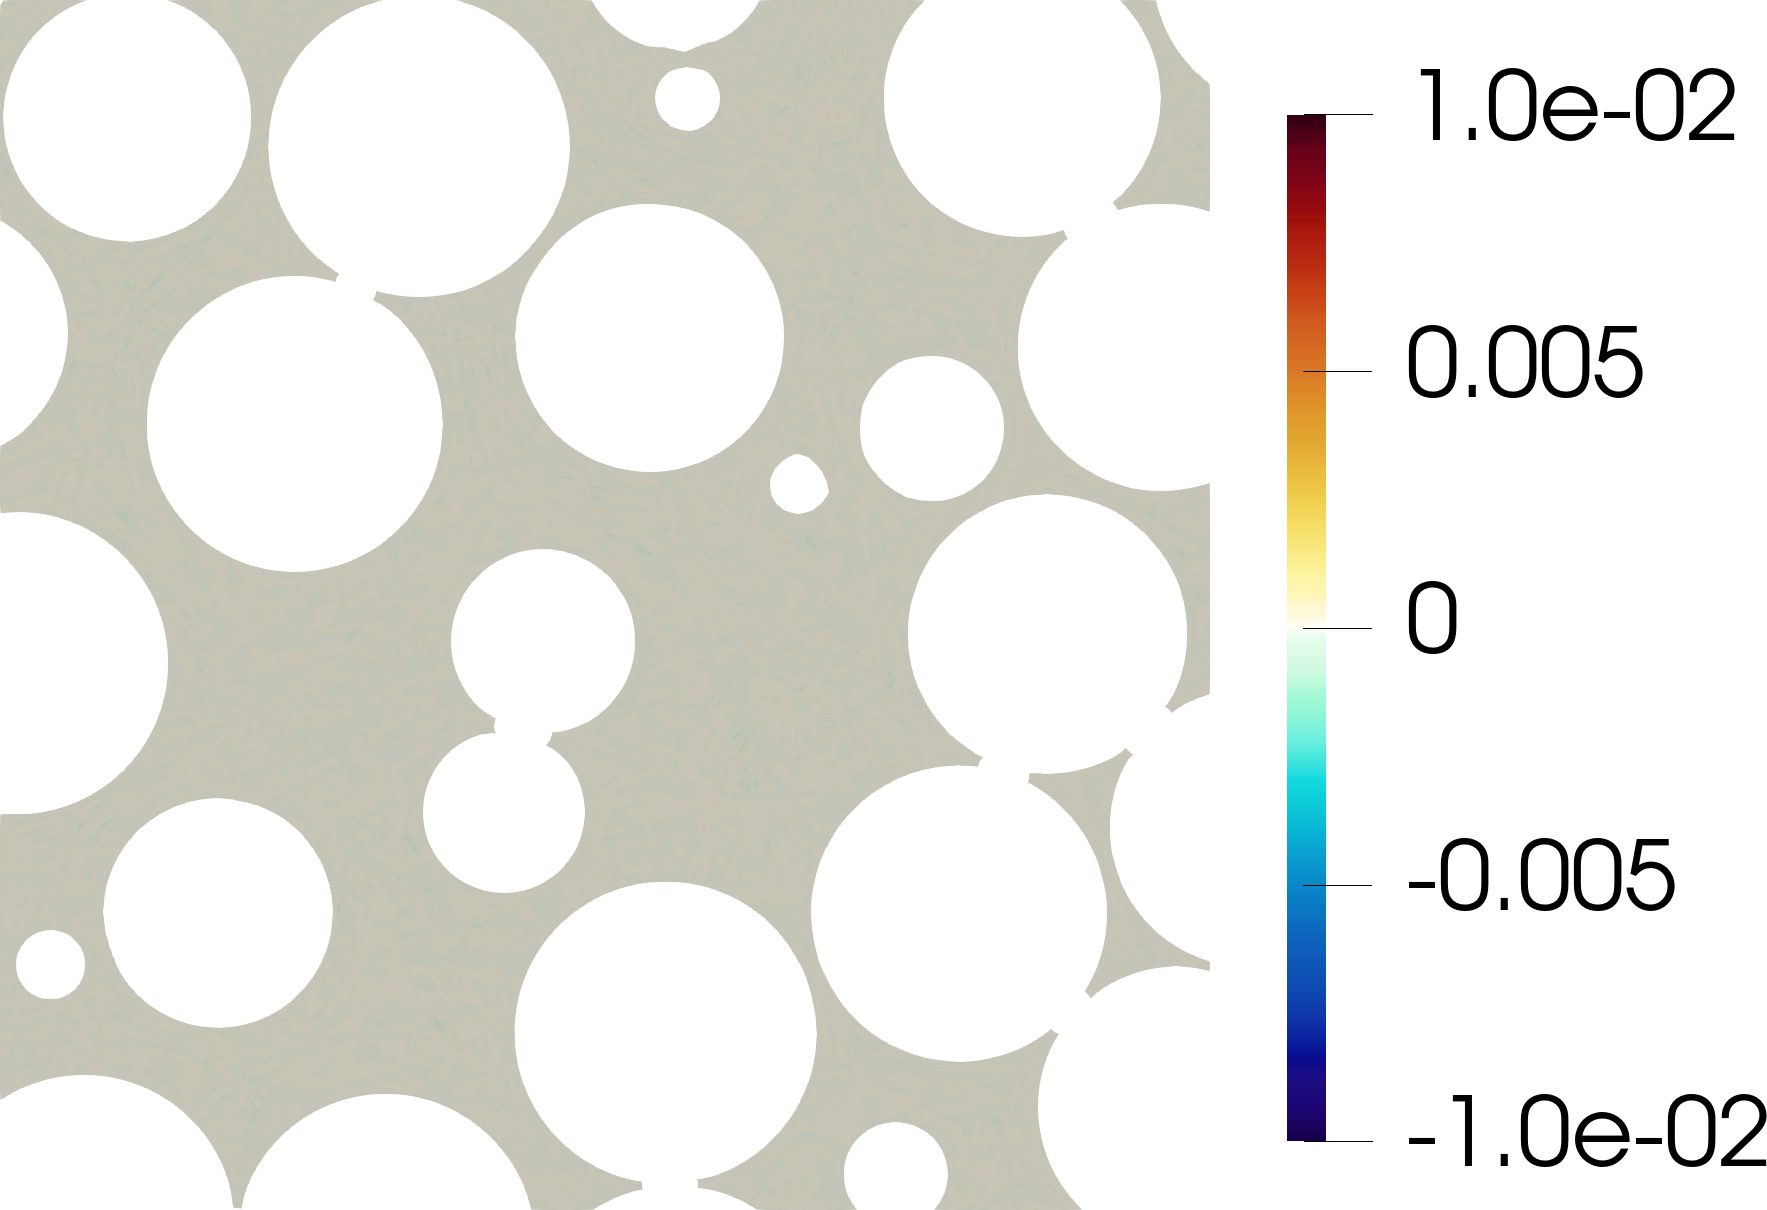
\includegraphics[width=\linewidth]{figs/7/mrcz err.png}
    \caption{MRCZ}
  \end{subfigure}
  \hfill
  \begin{subfigure}[t]{0.30\linewidth}
    \centering
    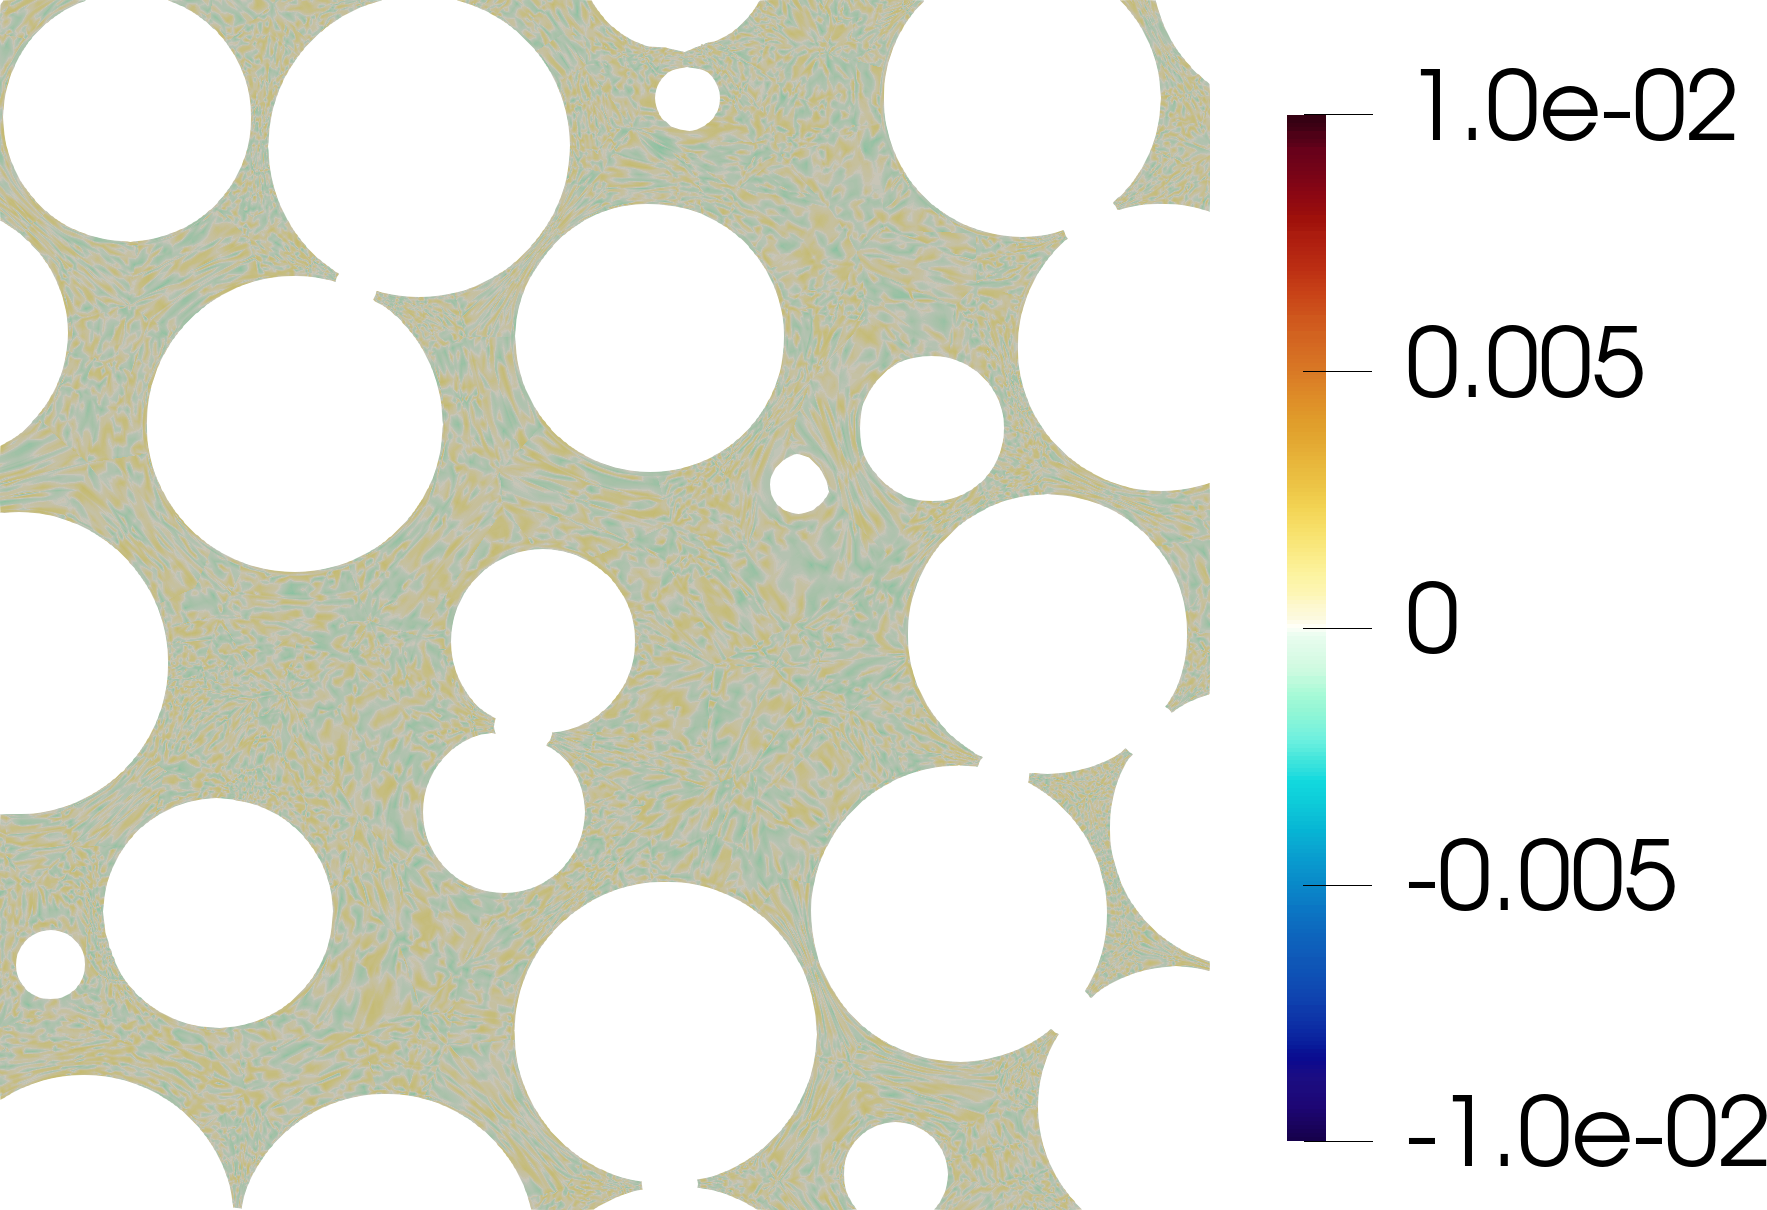
\includegraphics[width=\linewidth]{figs/7/sz3nekrs err.png}
    \caption{FDWZ}
  \end{subfigure}
  \hfill
  \begin{subfigure}[t]{0.30\linewidth}
    \centering
    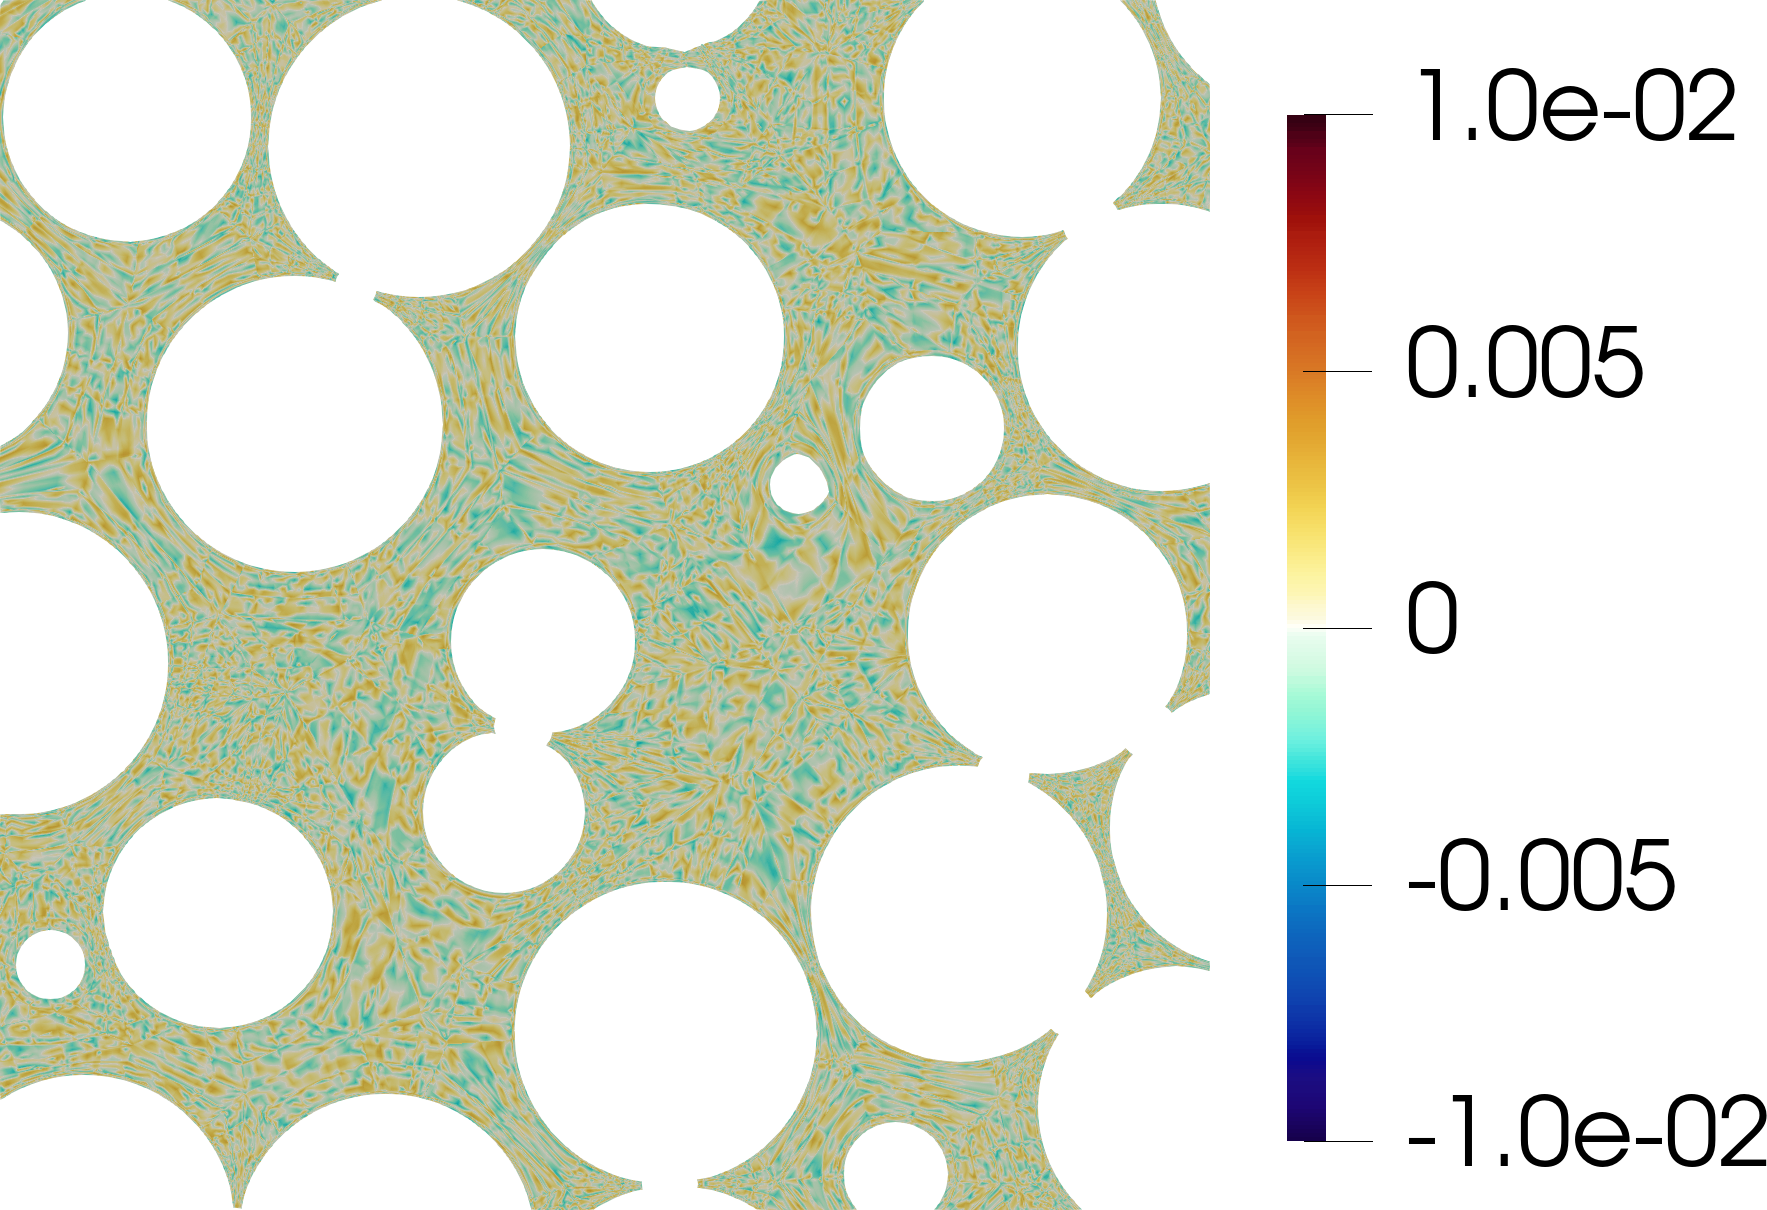
\includegraphics[width=\linewidth]{figs/7/sz3 err.png}
    \caption{SZ3-1}
  \end{subfigure}
  \\
  \begin{subfigure}[t]{0.30\linewidth}
    \centering
    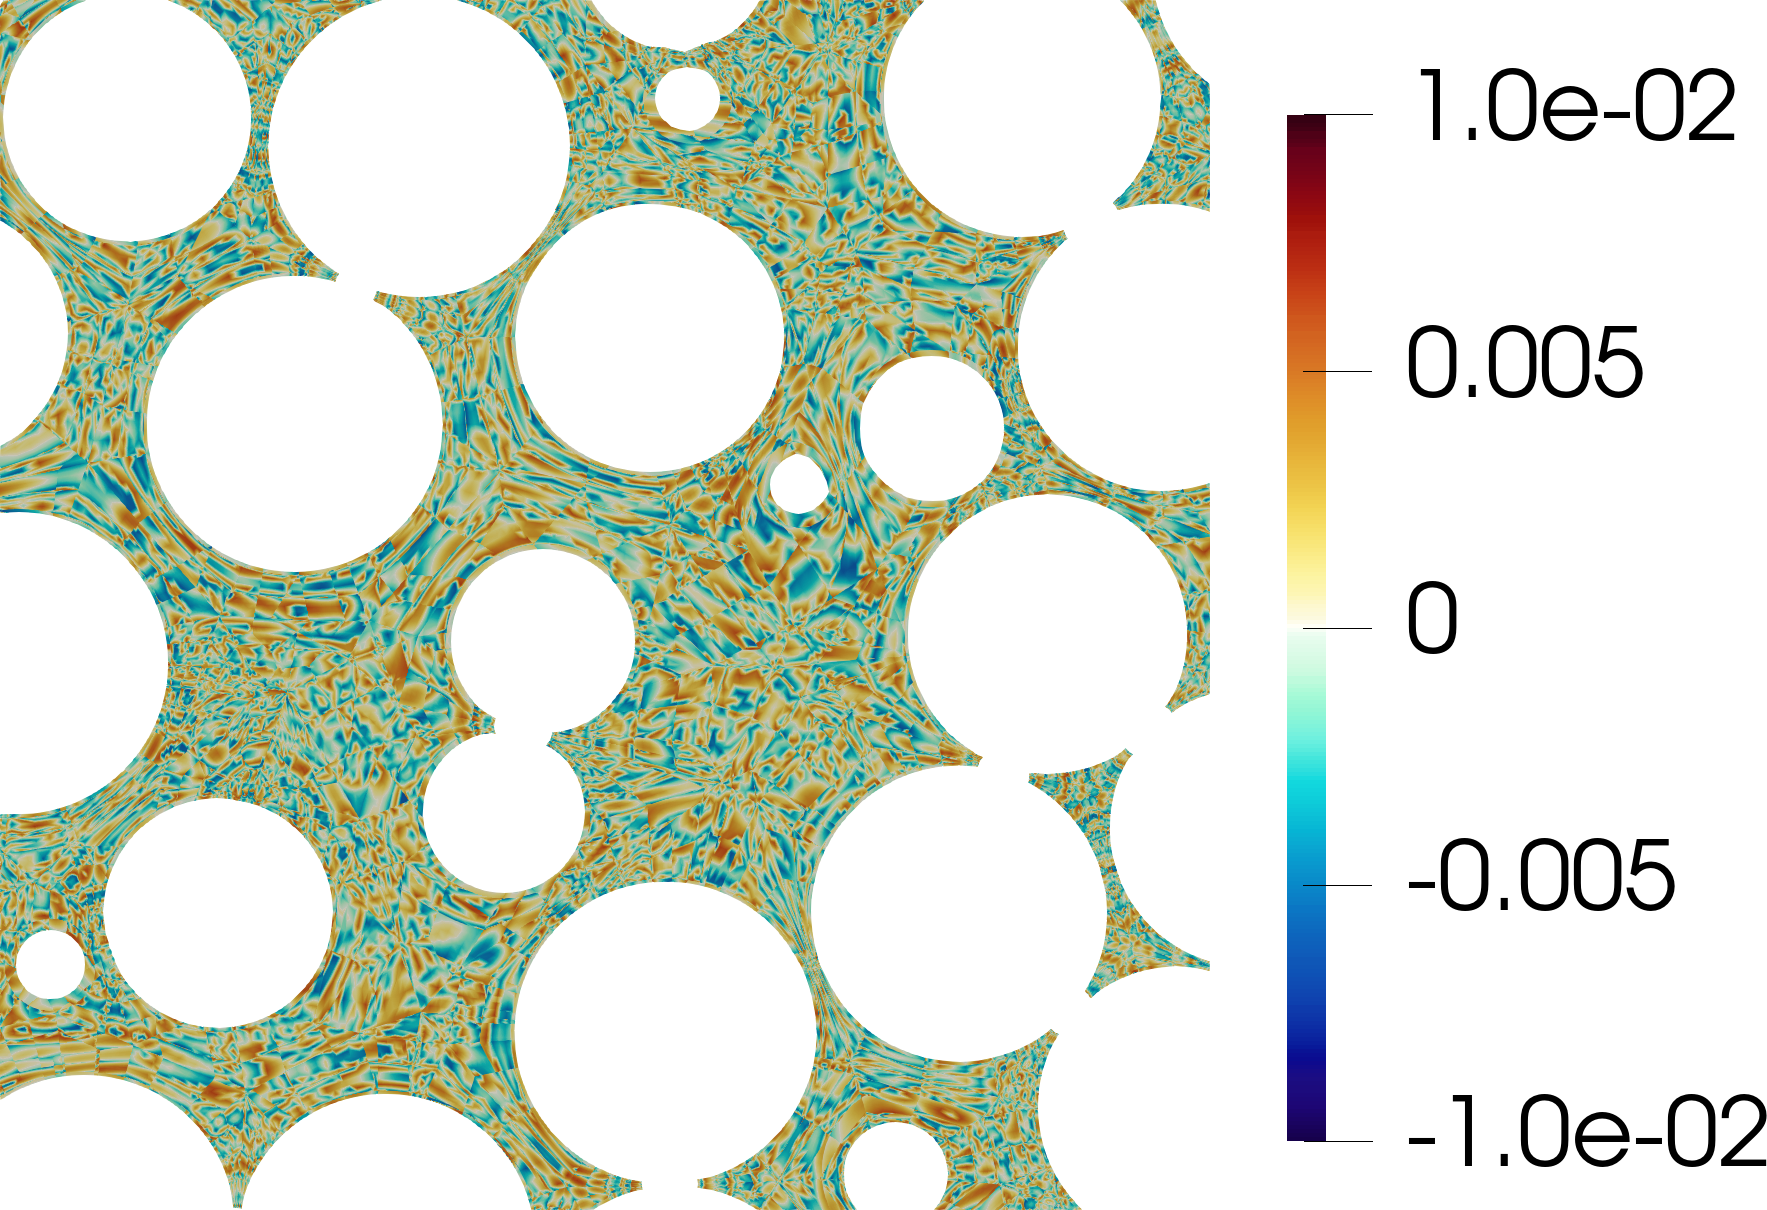
\includegraphics[width=\linewidth]{figs/7/sz2 err.png}
    \caption{SZ2-1}
  \end{subfigure}
  \hfill
  \begin{subfigure}[t]{0.30\linewidth}
    \centering
    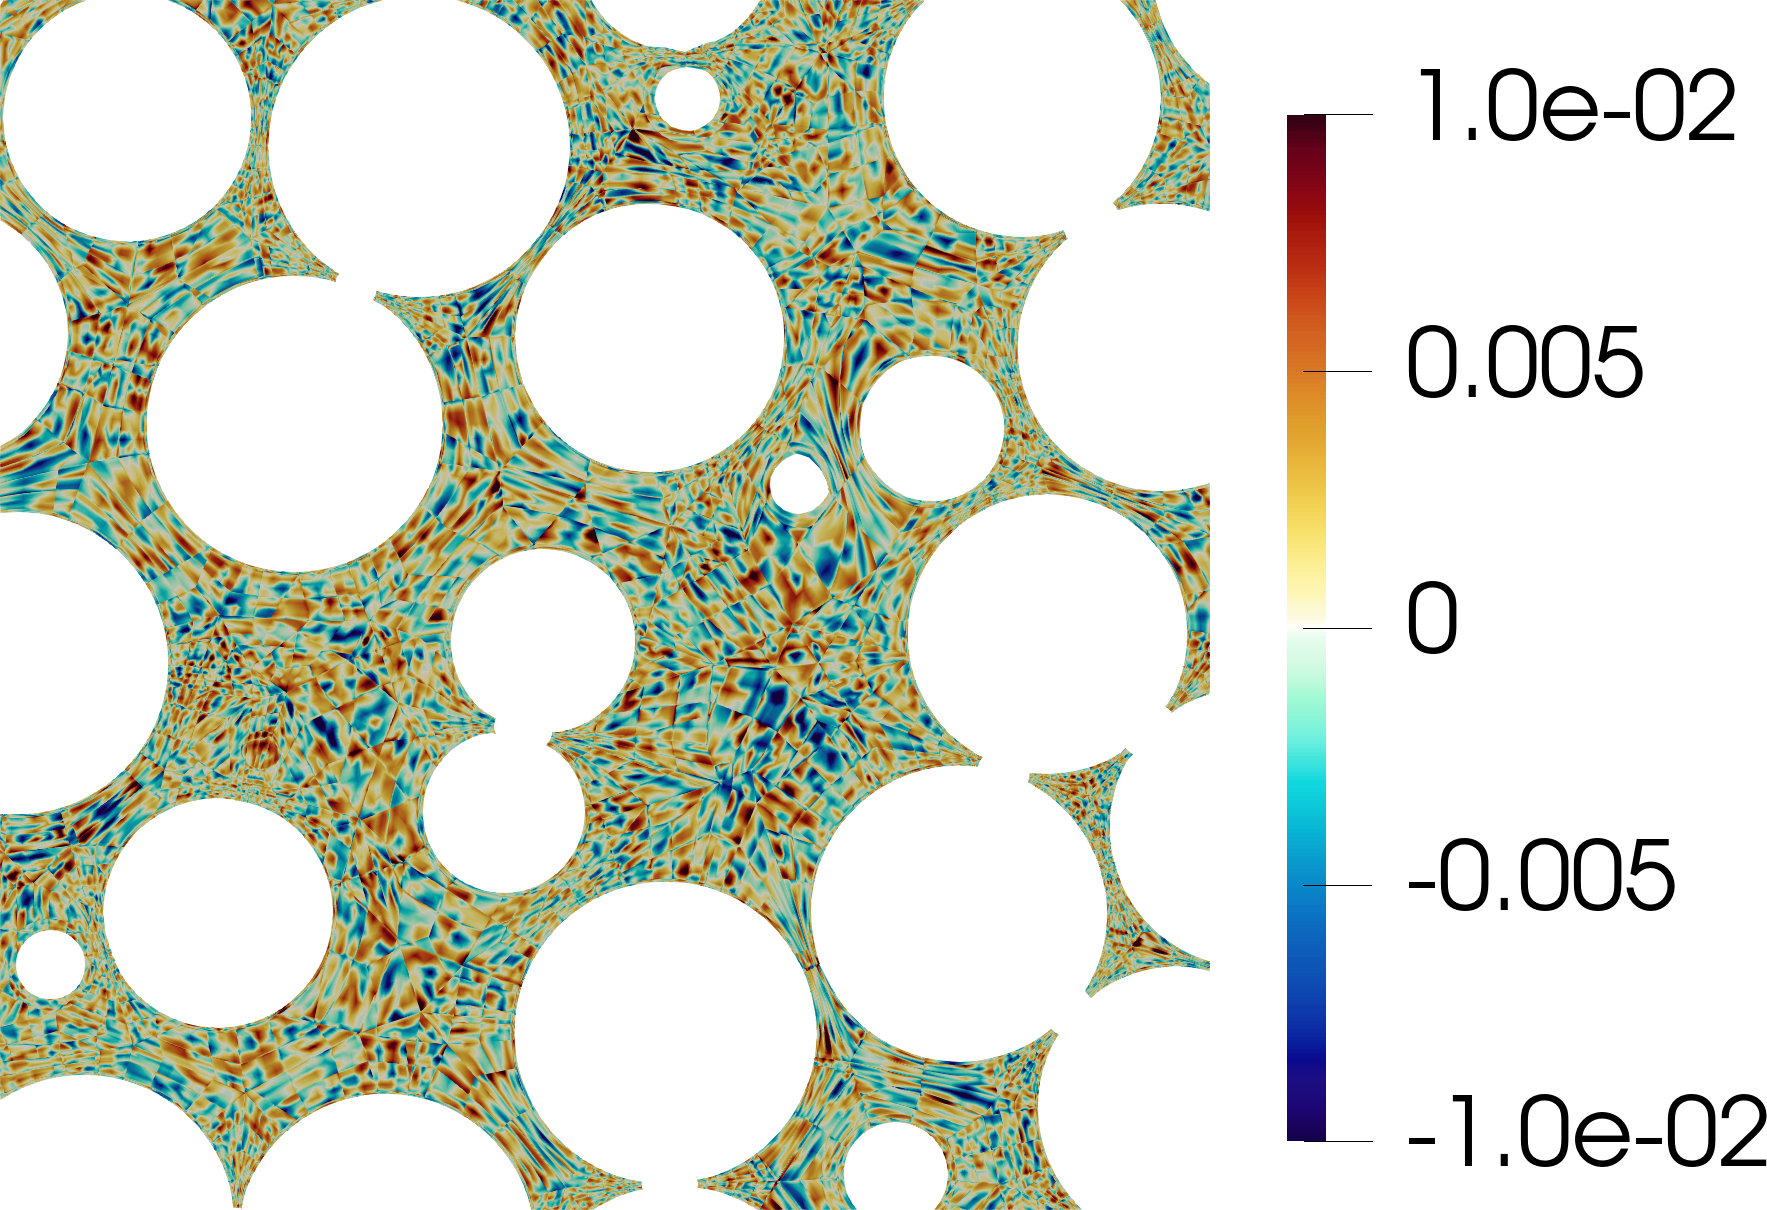
\includegraphics[width=\linewidth]{figs/7/zfp err.png}
    \caption{ZFP}
  \end{subfigure}
  \hfill
  \begin{subfigure}[t]{0.30\linewidth}
    \centering
    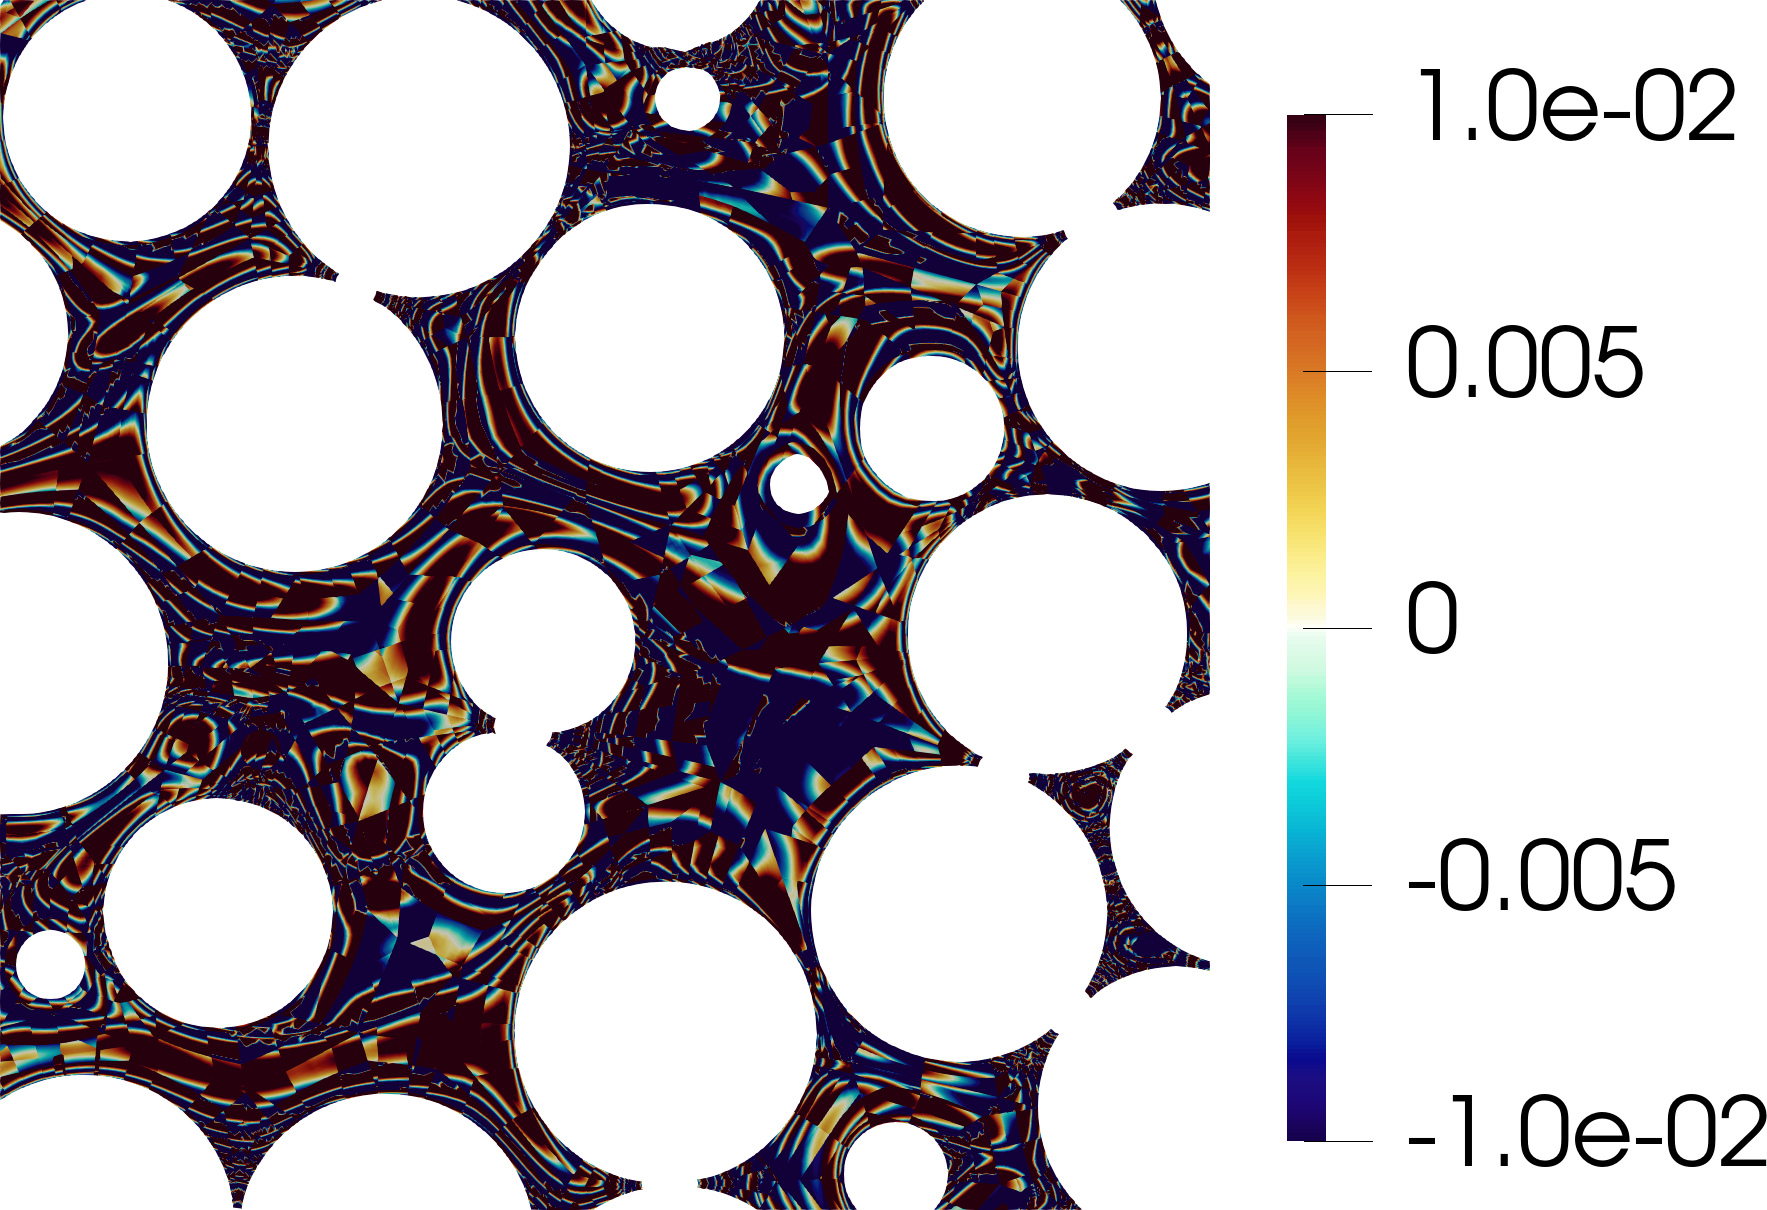
\includegraphics[width=\linewidth]{figs/7/sperr err.png}
    \caption{SPERR}
  \end{subfigure}
  \caption{Difference visualization of a slice of the Temperature field from data 4T. The compression ratios for all compressors are unified as $\sim$26.07 for a fair comparison.}
  \label{fig:distortion}
\end{figure}

Table~\ref{tab:error-bound-visualization} reports the error bounds selected for each compressor to achieve comparable compression ratios of approximately 26.07. Among the evaluated methods, MRCZ requires the tightest value-range-based relative error bound of $1.04\times10^{-4}$, whereas ZFP and SPERR require substantially larger error bounds of $3.16\times10^{-1}$ and $4.52\times10^{-2}$, respectively.

The corresponding pointwise reconstruction errors are visualized in Figure~\ref{fig:distortion}. MRCZ achieves the highest reconstruction fidelity, followed by FDWZ, while the baseline compressors exhibit more extensive errors.
